%!TEX output_directory = tmp
\documentclass[11pt, aspectratio=169]{beamer}
\usepackage[utf8]{inputenc}
\usepackage[russian]{babel}
\usepackage{subcaption}
\usepackage{ITMOtemplate}

\usepackage{algorithm,algpseudocode}
\usepackage{animate}

\newcommand{\R}{\mathbb{R}}
\pdfstringdefDisableCommands{\let\uppercase\@firstofone}

\graphicspath{{figs/}}

\newcommand{\Code}[1]{\textbf{#1}}
\newcommand{\bb}[1]{\mathbb{#1}}
\newcommand{\cc}[1]{\mathcal{#1}}

% Gif on fly convertation
\makeatletter
    \newcommand{\anim}[5][loop,autoplay,width=1.0\linewidth]{%
    \filename@parse{#3}%
    \edef\basefilename{\filename@area\filename@base}%
    \edef\basenewfilename{\filename@area png_sets/\filename@base}%
    \fbox{\animategraphics[#1]{#2}{\basenewfilename-}{#4}{#5}}%
    }
\makeatother


\usepackage[svgnames]{xcolor}
\makeatletter
    \newcommand{\colorboxed}[3][white]{\fcolorbox{#2}{#1}{\m@th$\displaystyle#3$}}
\makeatother


\newcommand{\SE}[1]{SE(#1)}
\newcommand{\SO}[1]{SO(#1)}
\newcommand{\R}{\mathbb{R}}

\algnewcommand{\IIf}[1]{\State\algorithmicif\ #1\ \algorithmicthen}
\algnewcommand{\EndIIf}{\unskip\ \algorithmicend\ \algorithmicif}

\title{\centering Исследование алгоритмов планирования\\ движения роботов с кинематическими\\ ограничениями}

\author[Author, Another]{
    \hfill
    {\bf Антипов В.А.}\inst{1}
    \hfill
}

\institute[ITMO University] % (optional, but mostly needed)
{
    \hfill
    \begin{minipage}[t]{0.4\textwidth}
        \centering{\inst{1}%
        ITMO University}
    \end{minipage}
    \hfill
 }

\date[Occasion]{\today }

\begin{document}

\frame{\titlepage}

\section{Введение}

\begin{frame}{Актуальность}
    \begin{columns}[onlytextwidth]
        \begin{column}{0.42\textwidth}
            \begin{figure}[ht]
                \centering
                % \animategraphics[loop,autoplay,width=1.0\linewidth]{10}{figures/gifs/orientc-}{0}{36}
                \caption{Планирование пути в Евклидовом пространстве}
            \end{figure}
        \end{column}
        \begin{column}{0.1\textwidth}
            \vspace{4cm}
            $\Rightarrow$
        \end{column}
        \begin{column}{0.42\textwidth}
            \begin{figure}[ht]
                \centering
                % \animategraphics[loop,autoplay,width=1.0\linewidth]{10}{figures/gifs/planec-}{0}{38}
                \caption{Планирование пути с учетом кинематических ограничений}
            \end{figure}
        \end{column}
    \end{columns}
    
\end{frame}

\begin{frame}{Планирование с ограничениями}
    \begin{figure}[ht]
        \centering
        % \animategraphics[loop,autoplay,width=0.45\linewidth]{10}{figures/gifs/linec2-}{0}{33}
        \caption{Необходимость использования конфигурационного пространства}
    \end{figure}
\end{frame}

\begin{frame}{Мотивация}
    \begin{figure}[ht]
        \begin{subfigure}[b]{0.48\textwidth}
            \centering
            % \animategraphics[loop,autoplay,width=1.0\linewidth]{20}{figures/gifs/7dof-hit-}{0}{270}
            \caption{iiwa 7dof player}
            \label{fig:rozum}
        \end{subfigure}
        \begin{subfigure}[b]{0.48\textwidth}
            \centering
            \anim[loop,autoplay,width=1.0\linewidth]{20}{figures/gifs/3dof-hit.gif}{0}{270}
            \caption{3dof player}
            \label{fig:ur}
        \end{subfigure}
        \caption{AirHockey Challenge}
    \end{figure}
\end{frame}

\begin{frame}{Цели и задачи ВКР}
    \begin{columns}[onlytextwidth]
        \begin{column}{0.4\textwidth}
            \begin{figure}[ht]
                \centering
                % \animategraphics[loop,autoplay,width=1.0\linewidth]{10}{figures/gifs/orientc-}{0}{36}
                \caption{Планирование пути с учетом кинематических ограничений}
            \end{figure}
        \end{column}
        \begin{column}{0.6\textwidth}
            \begin{itemize}
                \item Провести аналитический обзор методов
                \item Разработать среда моделирования для тестирования алгоритмов
                \item Реализовать не менее 3 алгоритмов планирования пути для роботов с кинематическими ограничениями
                \item Сравнить эффективность алгоритмов и выработать рекомендации по выбору  и настройке алгоритма
            \end{itemize}
        \end{column}
    \end{columns}
\end{frame}

\section{Постановка проблемы}

\begin{frame}{Планирование пути}
    \begin{columns}[onlytextwidth]
        \begin{column}{0.33\textwidth}
            \begin{figure}
                \centering
                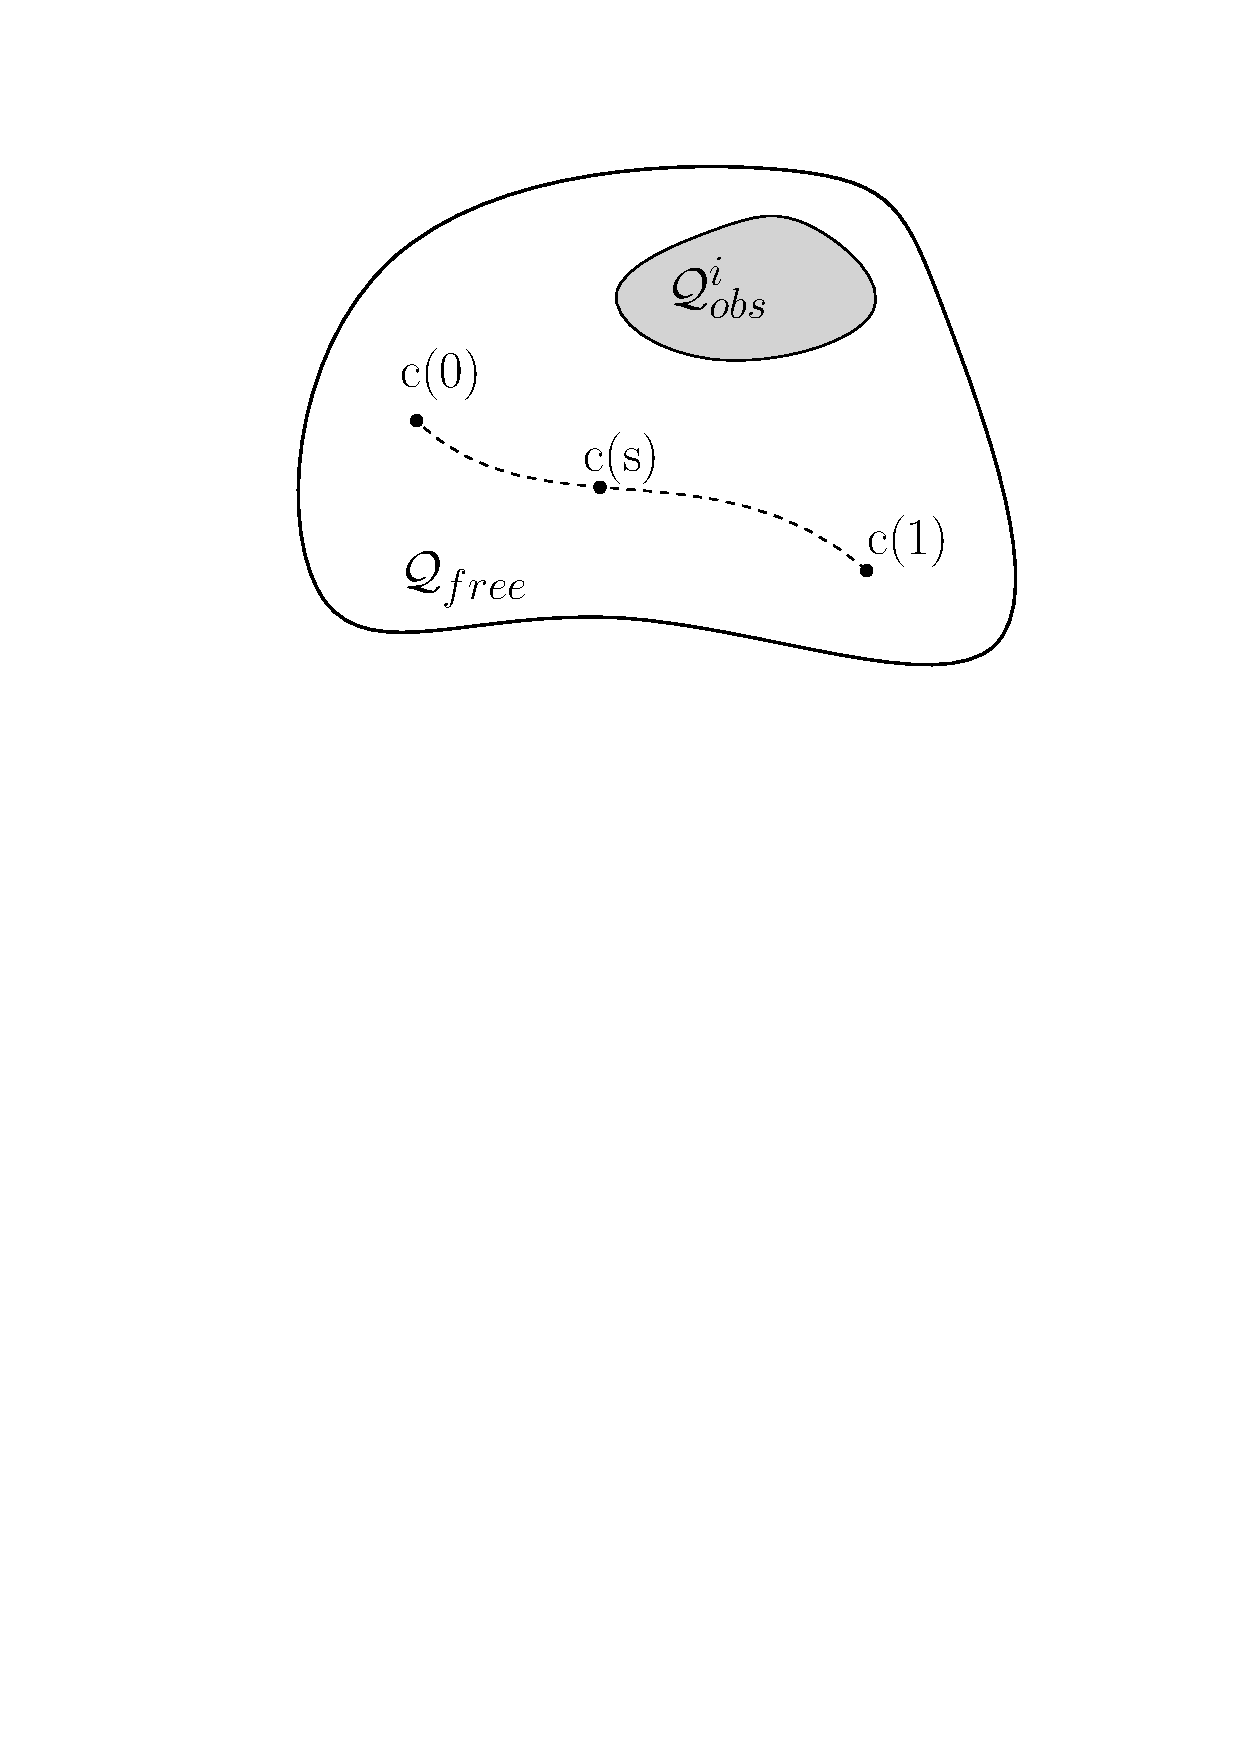
\includegraphics[width=\textwidth]{figures/graph/configuration_space.pdf}
                \caption{Пространство планирования}
                \label{fig:my_label}
            \end{figure}
        \end{column}
        \begin{column}{0.60\textwidth}
            Необходимо найти непрерывный путь удовлетворяющий краевым условиям:
            \begin{equation}
                c : [0, 1] \rightarrow \mathcal{Q}_{free},\quad  \begin{cases}q_{start} = c(0) \in \mathcal{Q}_{free}\\ q_{end} = c(1) \in \mathcal{Q}_{free} \\  c(s)\in \mathcal{Q}_{free},\ \forall s\in[0, 1]\end{cases}
            \end{equation}
            где $q \in \mathcal{Q}$ --- конфигурация, $\mathcal{Q}_{end}$ --- конфигурационное пространство, свободное от коллизий, заданных в операционном пространстве:
            \begin{equation}
                \mathcal{Q}_{free} = \left\{q\ |\ R(q) \cap \mathcal{W}_{free} \neq \emptyset\right\}
            \end{equation}
        \end{column}
    \end{columns}
\end{frame}

\begin{frame}{Планирование пути с ограничениями}
    В работе рассмотриваются только кинематические (голономные) ограничения
    \begin{columns}[onlytextwidth]
        \begin{column}{0.62\textwidth}
            \begin{alertblock}{Функция ограничений}
                \begin{equation}
                    \nonumber F : \mathcal{Q} \rightarrow \mathbb{R}^k  \iff \forall q\in \mathcal{Q}: F(q)=0
                \end{equation}
            \end{alertblock}
            \begin{alertblock}{Многообразие ограничений}
                \begin{equation}
                    \nonumber \mathcal{X} =\{q\in \mathcal{Q} | F(q)=0 \}
                \end{equation}
            \end{alertblock}
            Задача планирования глобального пути с ограничениями:
            \begin{equation}
                c : [0, 1] \rightarrow \mathcal{X}_{free},\   \begin{cases}q_{start} = c(0) \in \colorboxed{red}{\mathcal{X}_{free}}\\ q_{end} = c(1) \in \colorboxed{red}{\mathcal{X}_{free}} \\  c(s)\in \colorboxed{red}{\mathcal{X}_{free}},\ \forall s\in[0, 1]\end{cases}
            \end{equation}
        \end{column}
        \begin{column}{0.35\textwidth}
            \begin{figure}
                \centering
                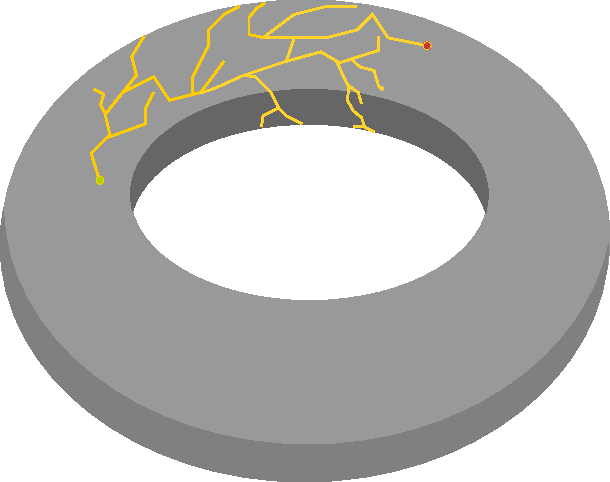
\includegraphics[width=\textwidth]{figures/graph/torus.pdf}
                \caption{Планирование пути на многообразии $\mathbb{T}^2$}
                \label{fig:my_label}
            \end{figure}
        \end{column}
    \end{columns}
\end{frame}

\section{Исследование методов}
\begin{frame}{Методы оптимального планирования}
    Sampling методы наиболее универсальны и не потдвержены проклятью размерности:
    \begin{figure}[ht]
        \begin{subfigure}[b]{0.48\textwidth}
            \centering
            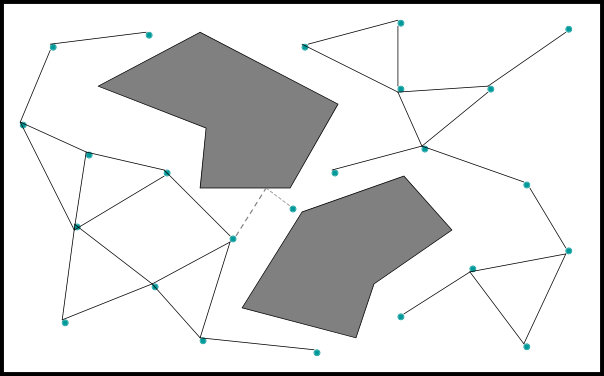
\includegraphics[width=0.9\textwidth]{figures/prm-example.png}
            \caption{PRM (Многозапросный)}
            \label{fig:prm-example}
        \end{subfigure}
        \begin{subfigure}[b]{0.48\textwidth}
            \centering
            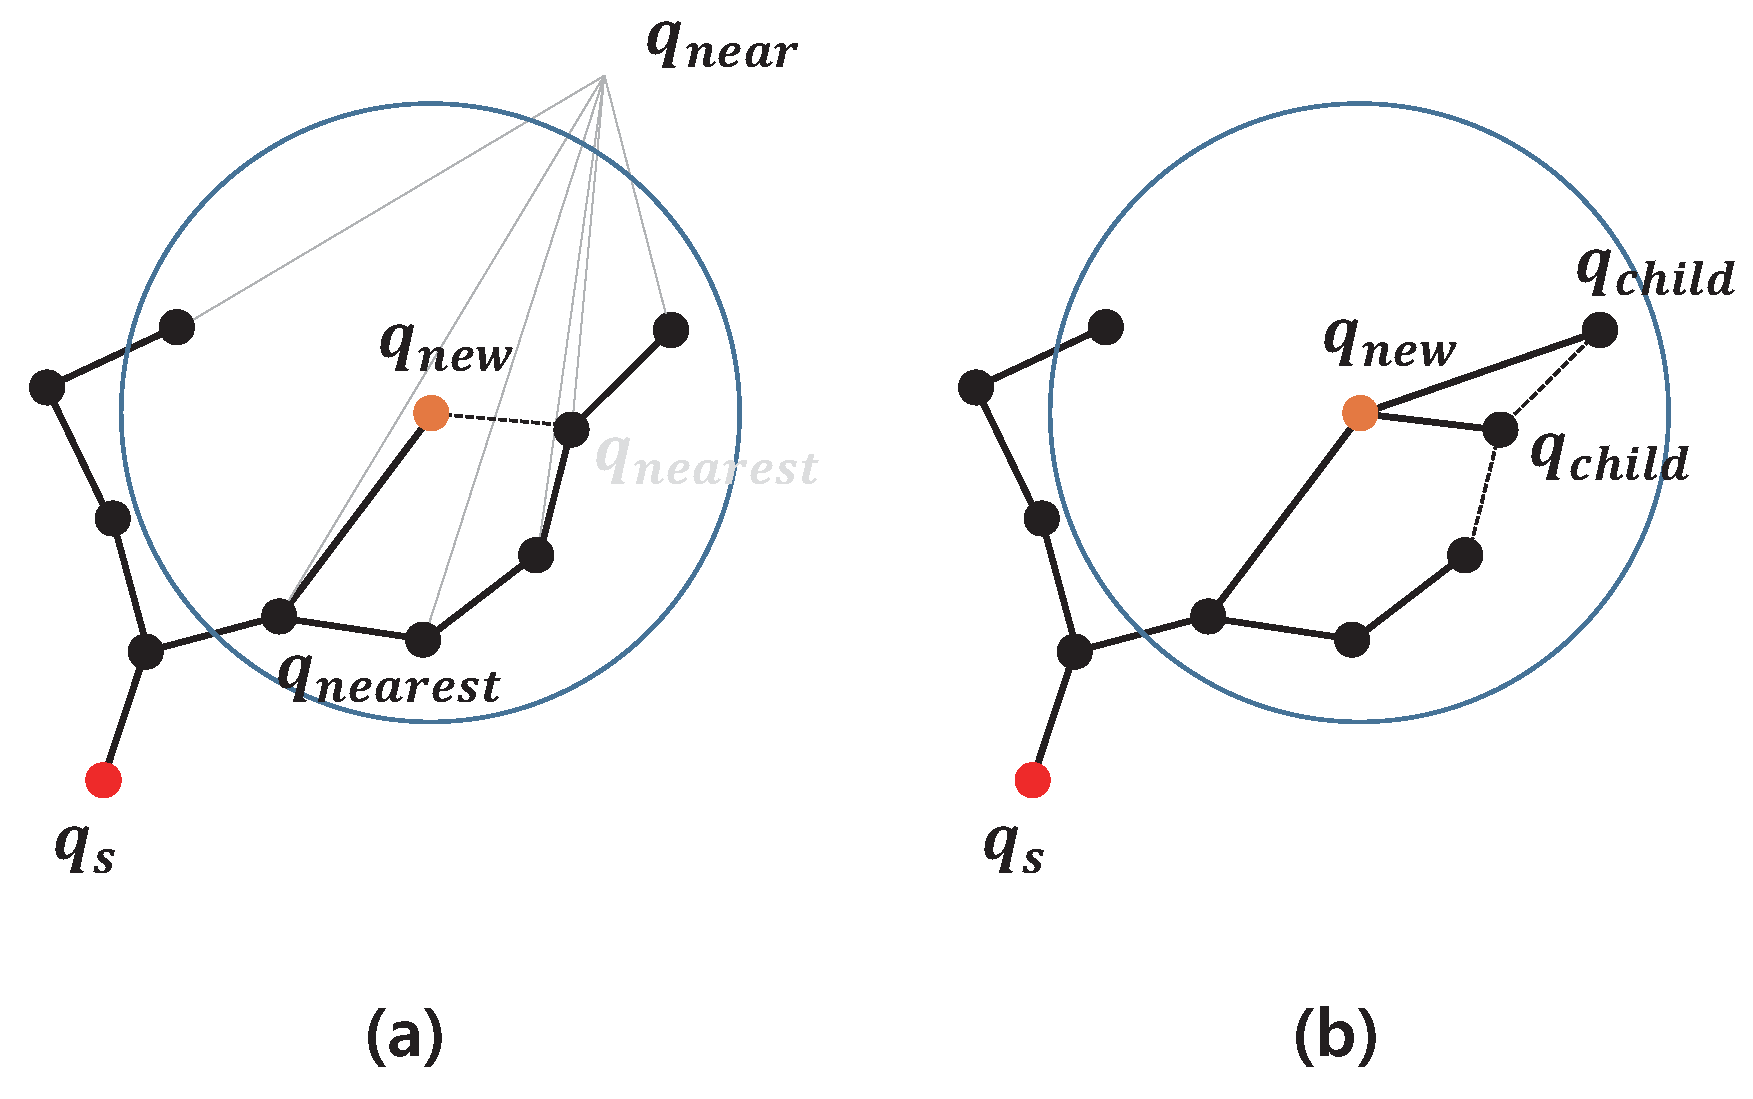
\includegraphics[width=0.9\textwidth]{figures/rrt-example.png}
            \caption{RRT (Однозапросный)}
            \label{fig:rrt-example}
        \end{subfigure}
        \caption{Методы на основе сэмплирования}
    \end{figure}
\end{frame}

\begin{frame}{Методы планирования c ограничениями}
    \begin{table}[ht]
        \begin{tabular}{|p{0.49\textwidth}|p{0.49\textwidth}|}
        \hline
        На основе методов проецирования & На основе метода продолжения по параметру\\
        \hline
        \begin{enumerate}
          \item \textbf{RGDRRT}: Randomized Gradient Descent
          \item \textbf{CBiRRT}: Constrained Bi-directional RRT
          \item \textbf{AG-CBiRRT}: Graph-based CBiRRT
        \end{enumerate} & \begin{enumerate}
          \item \textbf{ATACE}: Alternate Task-space And Configuration-space Exploration
          \item \textbf{HC-Planner}: Higher-dimensional Continuation planner
          \item \textbf{TBRRT}/\textbf{TSRRT}: Tangent bundle/space RRT
          \item \textbf{AtlasRRT}: Path Planning under Kinematic Constraints by Rapidly Exploring Manifolds
        \end{enumerate}\\
        \hline
        \end{tabular}
        \label{tab:constr_planning_review}
    \end{table}
\end{frame}


\begin{frame}{Разрешение ограничений}
    Для разрешения ограничений можно использовать проецирование:
    \begin{columns}[onlytextwidth]
        \begin{column}{0.6\textwidth}
            \leavevmode \only<1>{
                \begin{algorithm}[H]
                    \scriptsize
                    \caption{Метод Ньютона-Рафсона}\label{alg:newton-raphson}
                    \begin{algorithmic}[1]
                    \Procedure{CBiRRT\_projection}{}
                        \State $i = 0$
                        \State $x \gets F(q)$
                        \While {$\|x\|_2 > \epsilon$}
                        \IIf {$i > max\_iter$} \Return false 
                        \EndIIf
                        \State $q \gets q - J^+ x$
                        \State $x \gets F(q)$
                        \State $i\gets i+1$
                        \EndWhile
                        \State \Return $q$
                    \EndProcedure
                    \end{algorithmic}
                \end{algorithm} 
            }
            \leavevmode \only<2>{
                \begin{algorithm}[H]
                    \scriptsize
                    \caption{Метод Ньютона-Рафсона}\label{alg:newton-raphson}
                    \begin{algorithmic}[1]
                    \Procedure{CBiRRT\_projection}{}
                        \State $i = 0$
                        \State $x \gets F(q)$
                        \While {$\|x\|_2 > \epsilon$}
                        \IIf {$i > max\_iter$} 
                            \Return false
                        \EndIIf
                        \State $q \gets q - \colorboxed{red}{J^+} x$
                        \State $x \gets F(q)$
                        \State $i\gets i+1$
                        \EndWhile
                        \State \Return $q$
                    \EndProcedure
                    \end{algorithmic}
                \end{algorithm}
            }
        \end{column}
        \begin{column}{0.39\textwidth}
            \begin{figure}
                \centering
                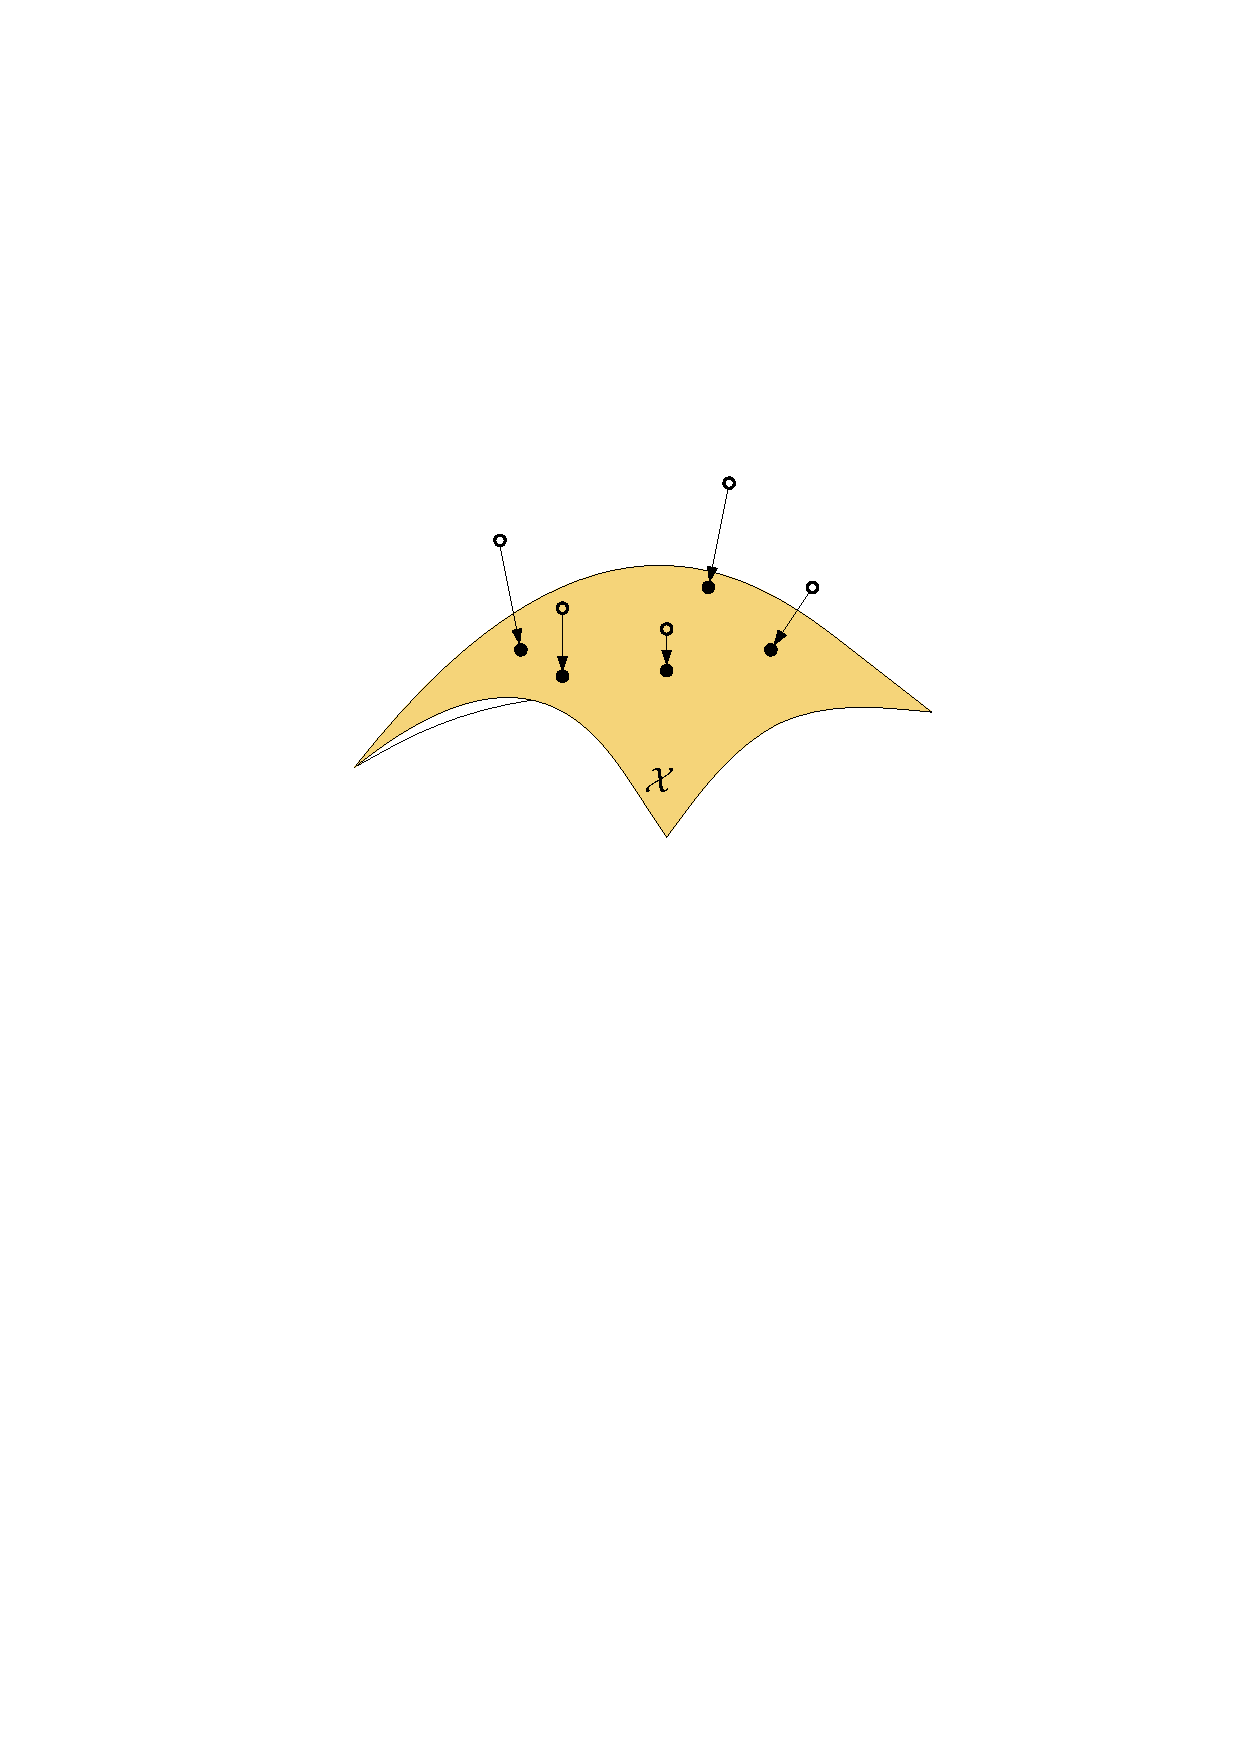
\includegraphics[width=1.0\textwidth]{figures/graph/projection.pdf}
                \caption{Проецирование сэмплов на многообразие ограничений}
                \label{fig:proj_sampling}
            \end{figure}
        \end{column}
    \end{columns}
    % \vspace{-0.5cm}
    где $J(q) = \dfrac{\partial F(q)}{\partial q}$ --- матрица Якоби функции ограничений.
\end{frame}

\begin{frame}{Разрешение ограничений}
    \begin{columns}[onlytextwidth]
        \begin{column}{0.4\textwidth}
            \textbf{Другой подход:} использование тангенциального пространства $T_q\mathcal{X}$
            \begin{figure}
                \centering
                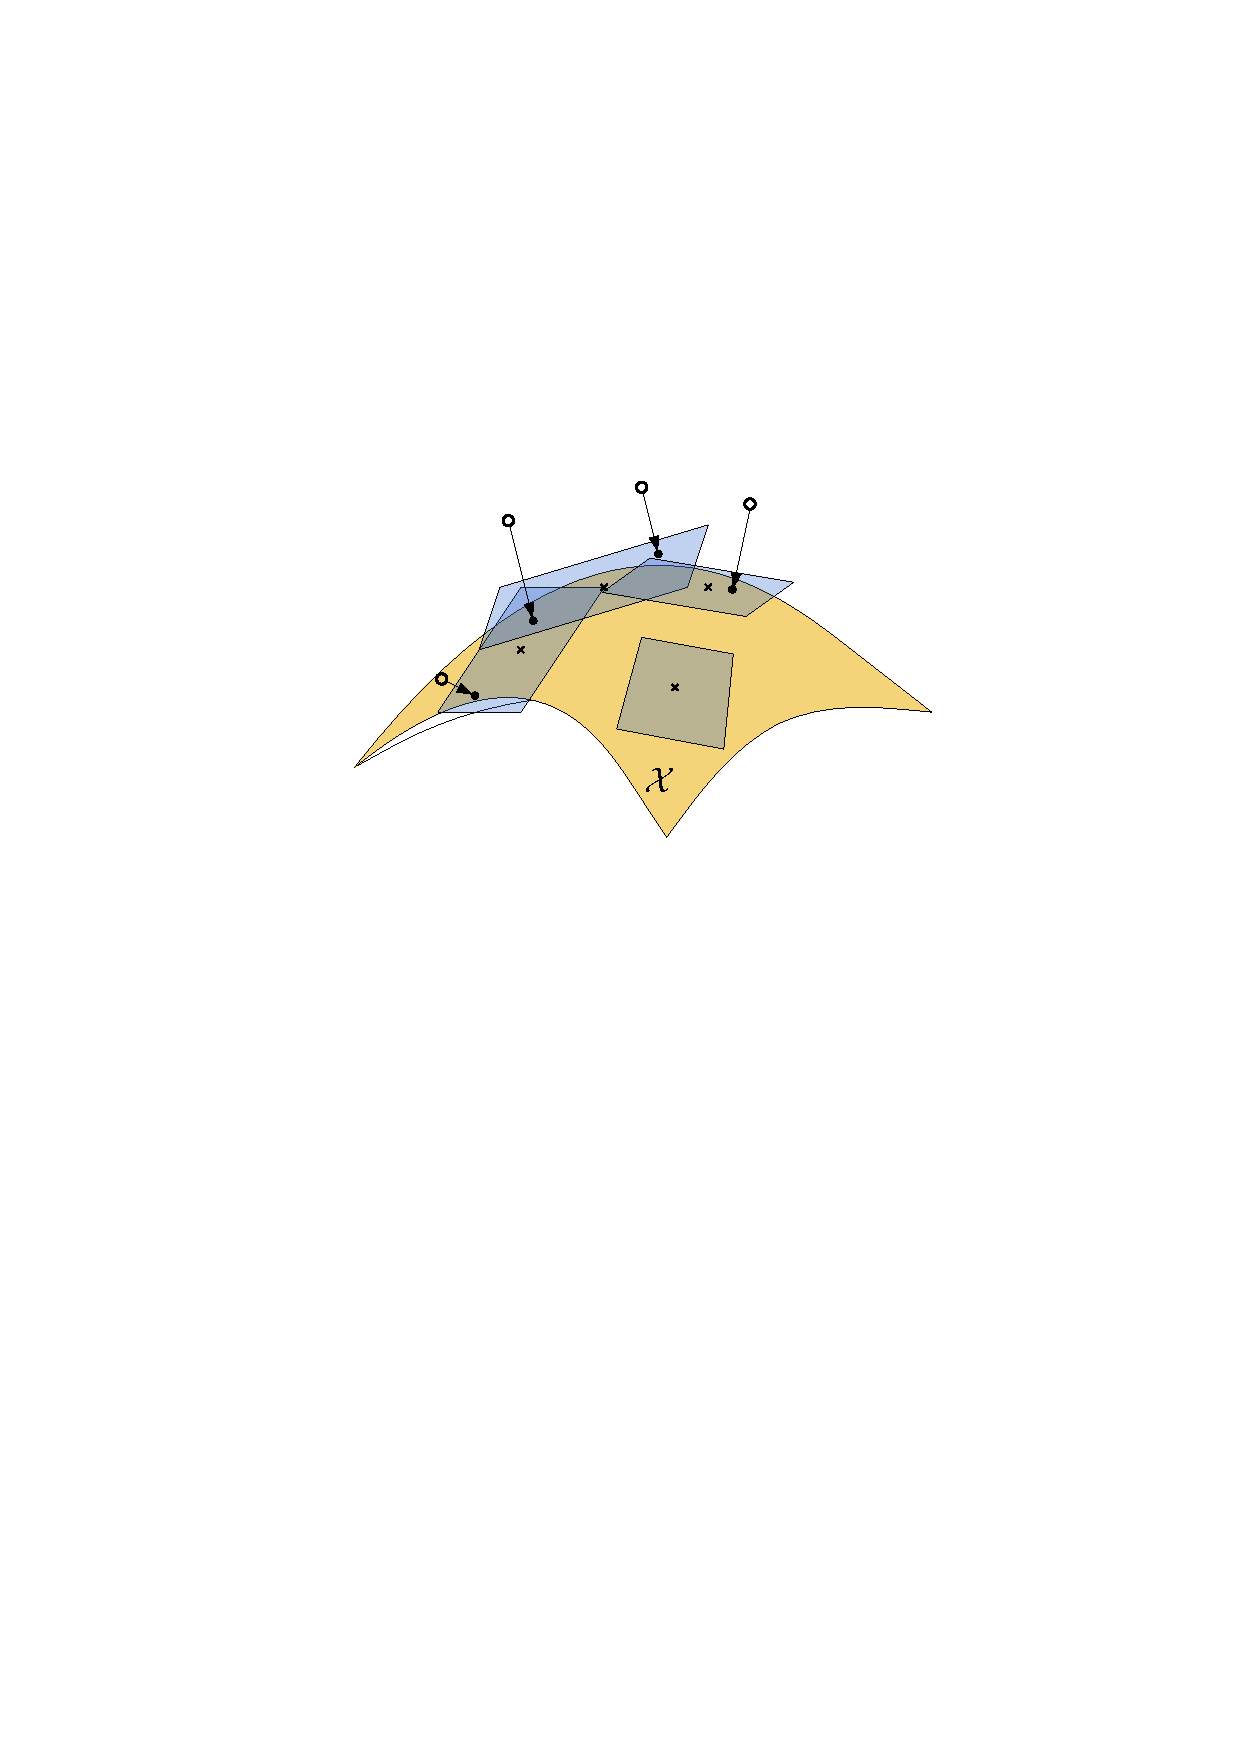
\includegraphics[width=1.0\textwidth]{figures/graph/tb_sampling.pdf}
                \caption{Сэмплирование в тангенциальном пространстве}
                \label{fig:tb_sampling}
            \end{figure}
        \end{column}
        \begin{column}{0.58\textwidth}
            \begin{algorithm}[H]
                \scriptsize
                \caption{TSRRT}\label{alg:TSRRT}
                \begin{algorithmic}[1]
                    \State TangentPlanes $T$
                    \State RRT.Init($q_{start}$, $q_{end}$, $T$)
                    \State TangentPlanes.Add(CreateTangentPlane($q_{start}$))
                    \State TangentPlanes.Add(CreateTangentPlane($q_{end}$))
                    \While{$i < I_{max}$}
                        \State $i \gets i + 1$
                        \State $T_i \gets $ SelectTangentPlane()
                        \State $q_{rand} \gets$ RandomSampleOnTangentPlane($T_i$)
                        \State $q_{new}\gets$ RRT.GetNewPoint($q_{rand}$)
                        \IIf{Connect($q_{near}$, $q_{new}$) != Success}
                            continue
                        \EndIIf
                        \If{Connect($q_{new}$, $q_{end}$) == Success}
                            \State \Return LazyProjection(RRT.ExtractPath())
                        \EndIf
                        \If{$\| F(q_{new})\|_2 > \epsilon$}
                            \State TangentPlanes.Add(CreateTangentPlane($q_{new}$))
                        \EndIf
                        \State RRT.ExtendTree($q_{near}, q_{new}$)
                    \EndWhile
                \end{algorithmic}
            \end{algorithm}
        \end{column}
    \end{columns}
\end{frame}

\begin{frame}{Разрешение ограничений}
    \begin{columns}[onlytextwidth]
        \begin{column}{0.4\textwidth}
            \textbf{Другой подход:} использование тангенциального пространства $T_q\mathcal{X}$
            \begin{figure}
                \centering
                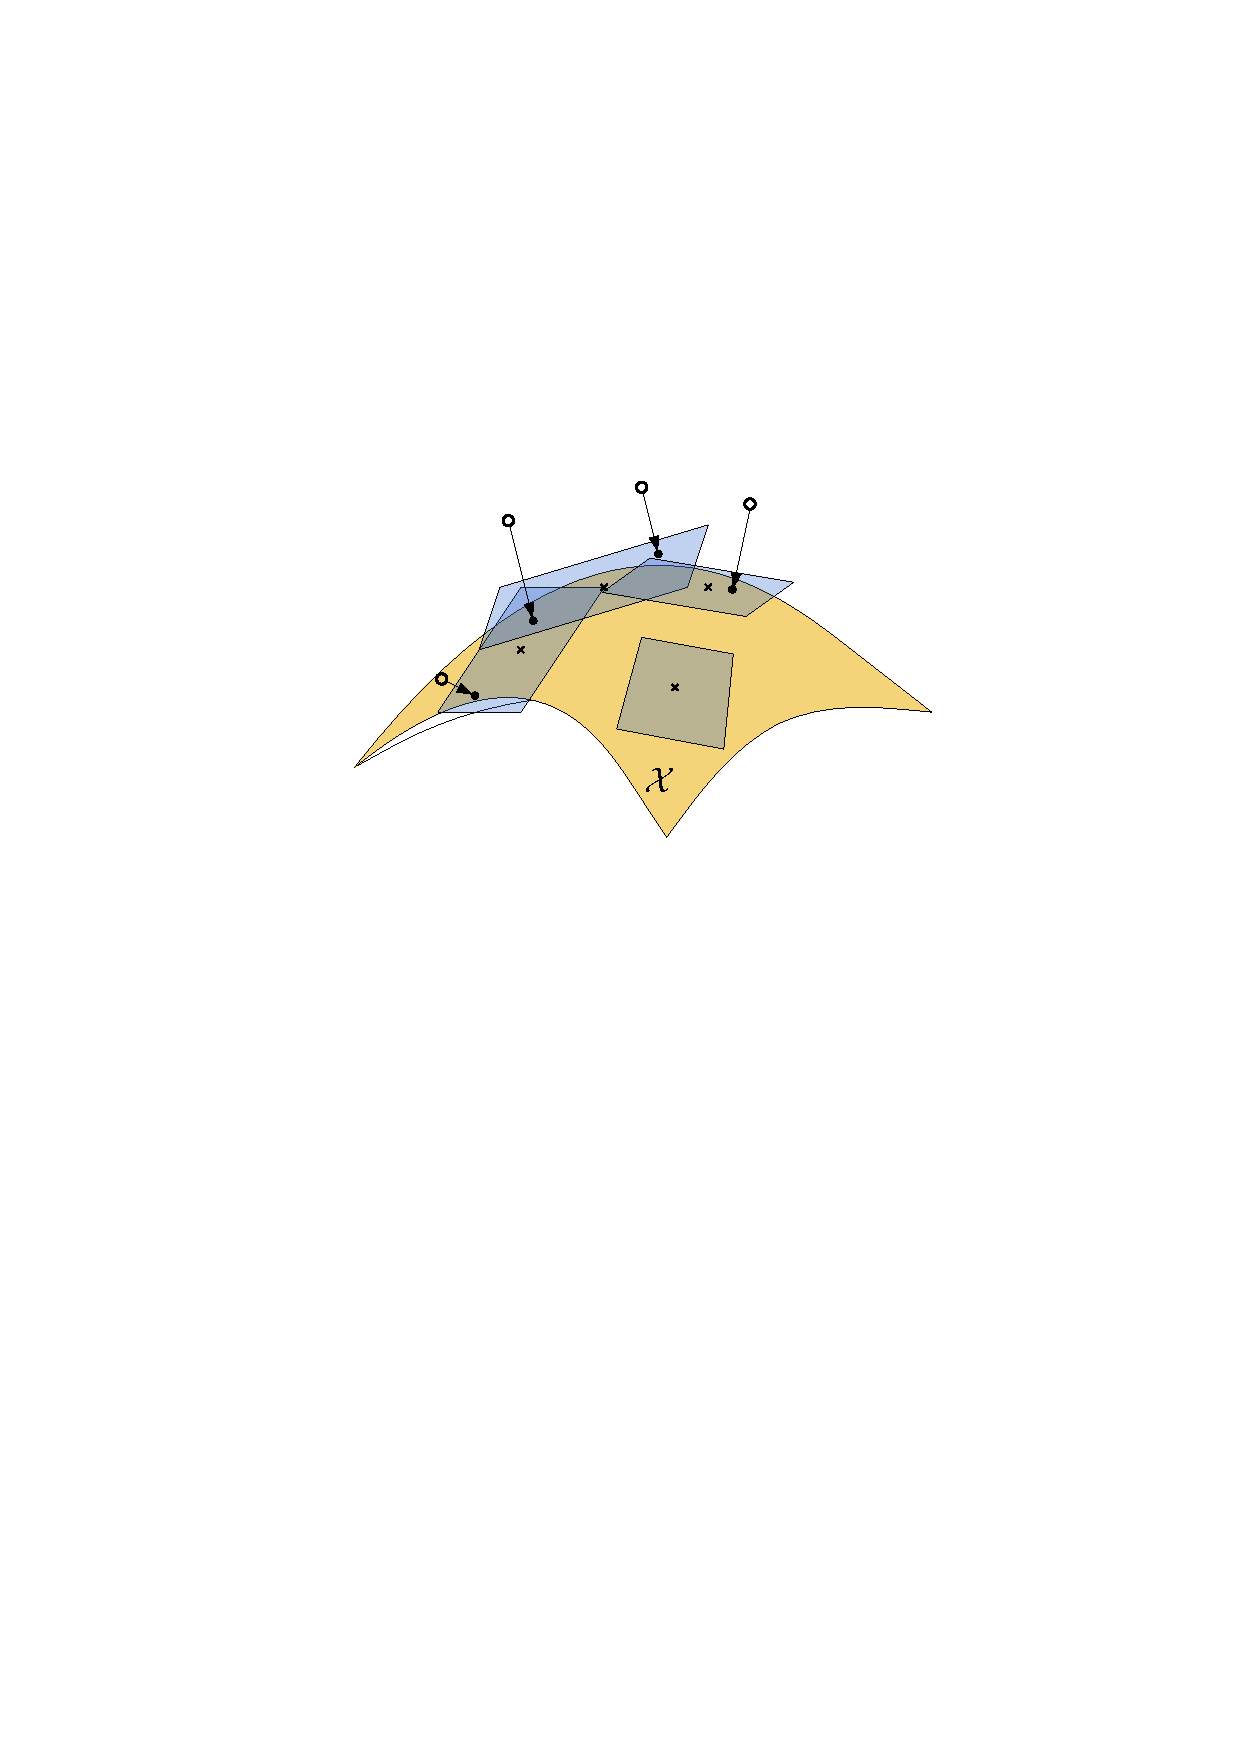
\includegraphics[width=1.0\textwidth]{figures/graph/tb_sampling.pdf}
                \caption{Сэмплирование в тангенциальном пространстве}
                \label{fig:tb_sampling}
            \end{figure}
        \end{column}
        \begin{column}{0.58\textwidth}
            \leavevmode \only<1>{
                \begin{alertblock}{Базис $T_q\mathcal{X}$}
                    \begin{align}
                        \begin{bmatrix}
                            J(q) \\ \Phi^T(q)
                        \end{bmatrix} \Phi(q) =
                        \begin{bmatrix}
                            0\\ I
                        \end{bmatrix}\\
                        \Rightarrow \Phi(q) = ker(J(q))
                    \end{align}
                \end{alertblock}
            }
            \leavevmode \only<2>{
                \begin{alertblock}{Базис $T_q\mathcal{X}$}
                    \begin{align}
                        \begin{bmatrix}
                            J(q) \\ \Phi^T(q)
                        \end{bmatrix} \colorboxed{orange}{\Phi(q)} =
                        \begin{bmatrix}
                            0\\ I
                        \end{bmatrix}\\
                        \Rightarrow \Phi(q) = ker(J(q))
                    \end{align}
                \end{alertblock}
            }
            % \leavevmode \only<3>{
            %     \begin{alertblock}{Базис $T_q\mathcal{X}$}
            %         \begin{equation}
            %             \begin{bmatrix}
            %                 J(q) \\ \Phi^T(q)
            %             \end{bmatrix} \colorboxed{orange}{\Phi(q)} =
            %             \begin{bmatrix}
            %                 0\\ I
            %             \end{bmatrix}
            %             \Rightarrow \Phi(q) = ker(J(q))
            %         \end{equation}
            %     \end{alertblock}
            %     \begin{alertblock}{Общий вид}
            %         \begin{equation}
            %             A = \begin{bmatrix}

            %             \end{bmatrix}, \quad
            %             \begin{bmatrix}
            %                 0\\ I
            %             \end{bmatrix}
            %             \Rightarrow \Phi(q) = ker(J(q))
            %         \end{equation}
            %     \end{alertblock}
            % }
        \end{column}
    \end{columns}
\end{frame}

\begin{frame}{Разрешение ограничений}
    Использование Атласа многообразия $\mathcal{A}_\mathcal{X}$ как пространства для планирования.
    \begin{columns}[onlytextwidth]
        \begin{column}{0.49\textwidth}
            \begin{figure}
                \centering
                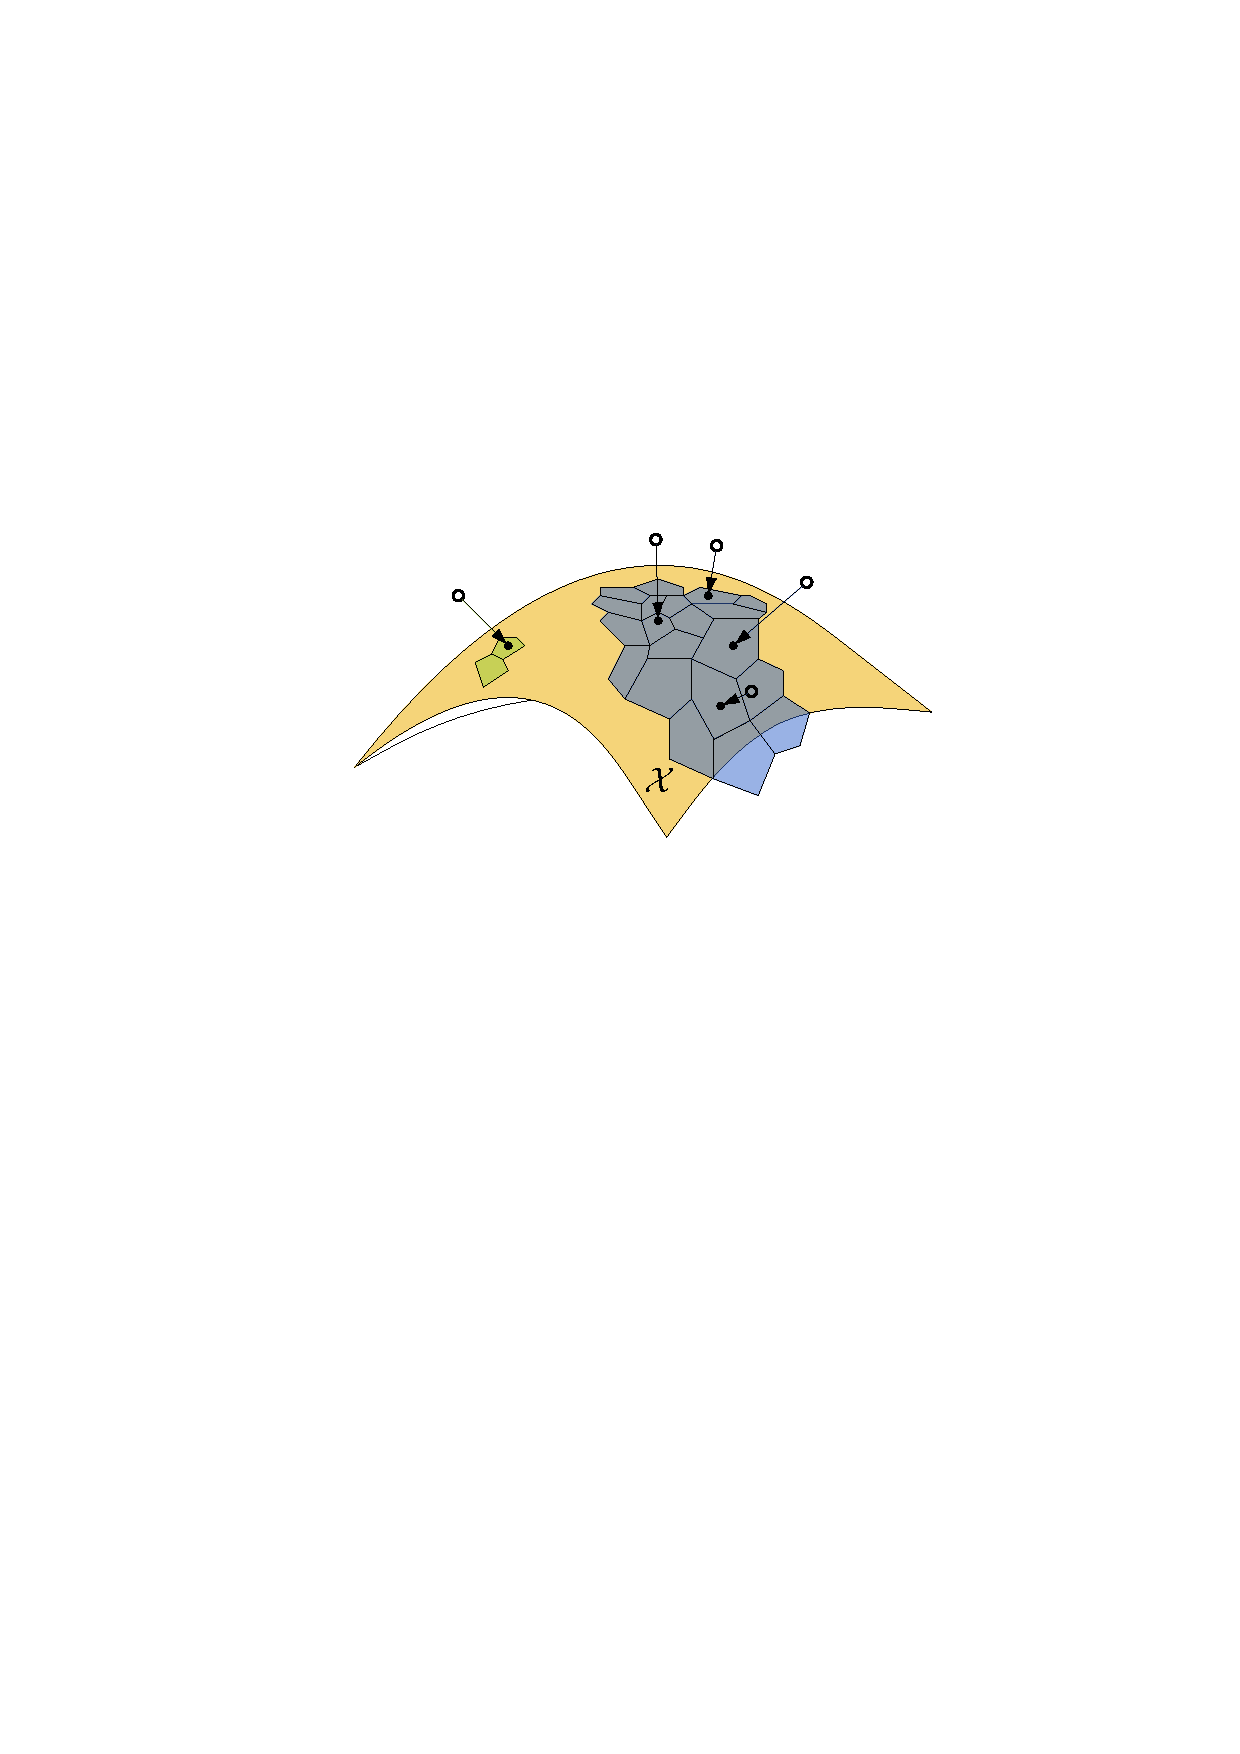
\includegraphics[width=1.0\textwidth]{figures/graph/atlas_sampling.pdf}
                \caption{Сэмплирование на Атласе}
                \label{fig:atlas_sampling}
            \end{figure}
        \end{column}
        \begin{column}{0.49\textwidth}
            \begin{figure}
                \centering
                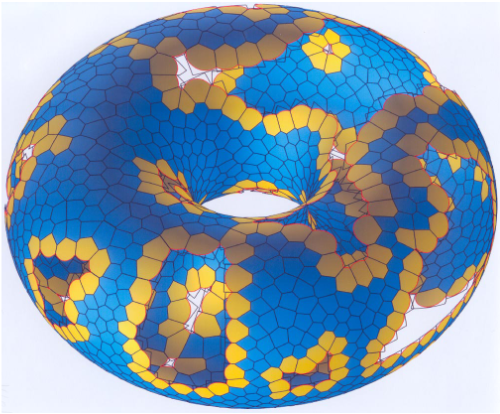
\includegraphics[width=0.7\textwidth]{figures/atlas_on_tor.png}
                \caption{Атлас $\mathbb{T}^2$}
                \label{fig:atlas_sampling}
            \end{figure}
        \end{column}
    \end{columns}
\end{frame}

\section{Среда моделирования}

\begin{frame}{Сцены моделирования}
    \begin{figure}[ht]
        \begin{subfigure}{0.32\textwidth}
            \centering
            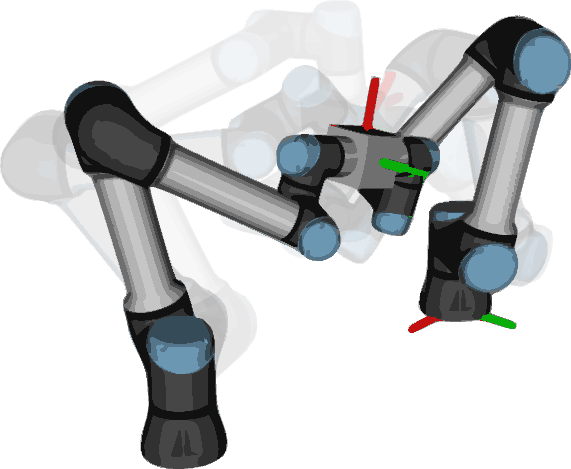
\includegraphics[width=1.0\textwidth]{figures/ur_coop.pdf}
            \caption{\centering Два манипулятора}
            \label{fig:ur_coop}
        \end{subfigure}
        \begin{subfigure}{0.32\textwidth}
            \centering
            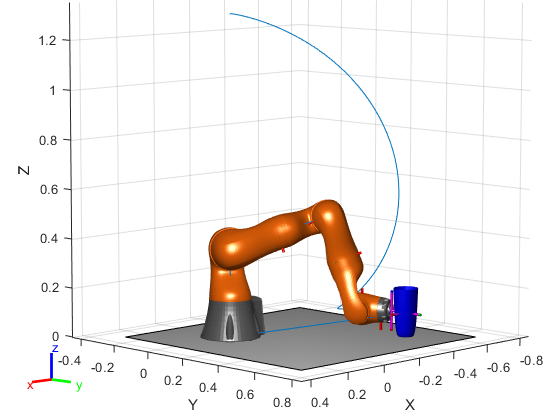
\includegraphics[width=1.0\textwidth]{figures/cup_constr.png}
            \caption{\centering Манипулирование кружкой с водой\\ \textbf{(В процессе)}}
            \label{fig:lbr_cup}
        \end{subfigure}
        \begin{subfigure}{0.32\textwidth}
            \centering
            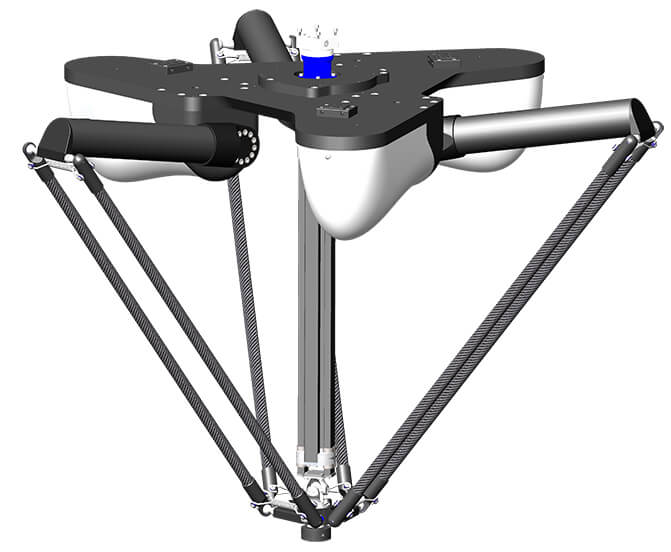
\includegraphics[width=1.0\textwidth]{figures/delta.png}
            \caption{\centering Параллельный манипулятор\\ \textbf{(В процессе)}}
            \label{fig:parallel}
        \end{subfigure}
        \label{fig:tasks}
        \caption{Задачи для тестирования}
    \end{figure}
\end{frame}


\begin{frame}{Два манипулятора}
    \begin{equation}
        F(q) = \psi^{-1}(w^{-1}_1(q)w_2(q)), \quad q = \begin{bmatrix} q_1 & q_2\end{bmatrix}
    \end{equation}
    \begin{columns}
        \begin{column}{0.55\textwidth}
            \begin{figure}
                \centering
                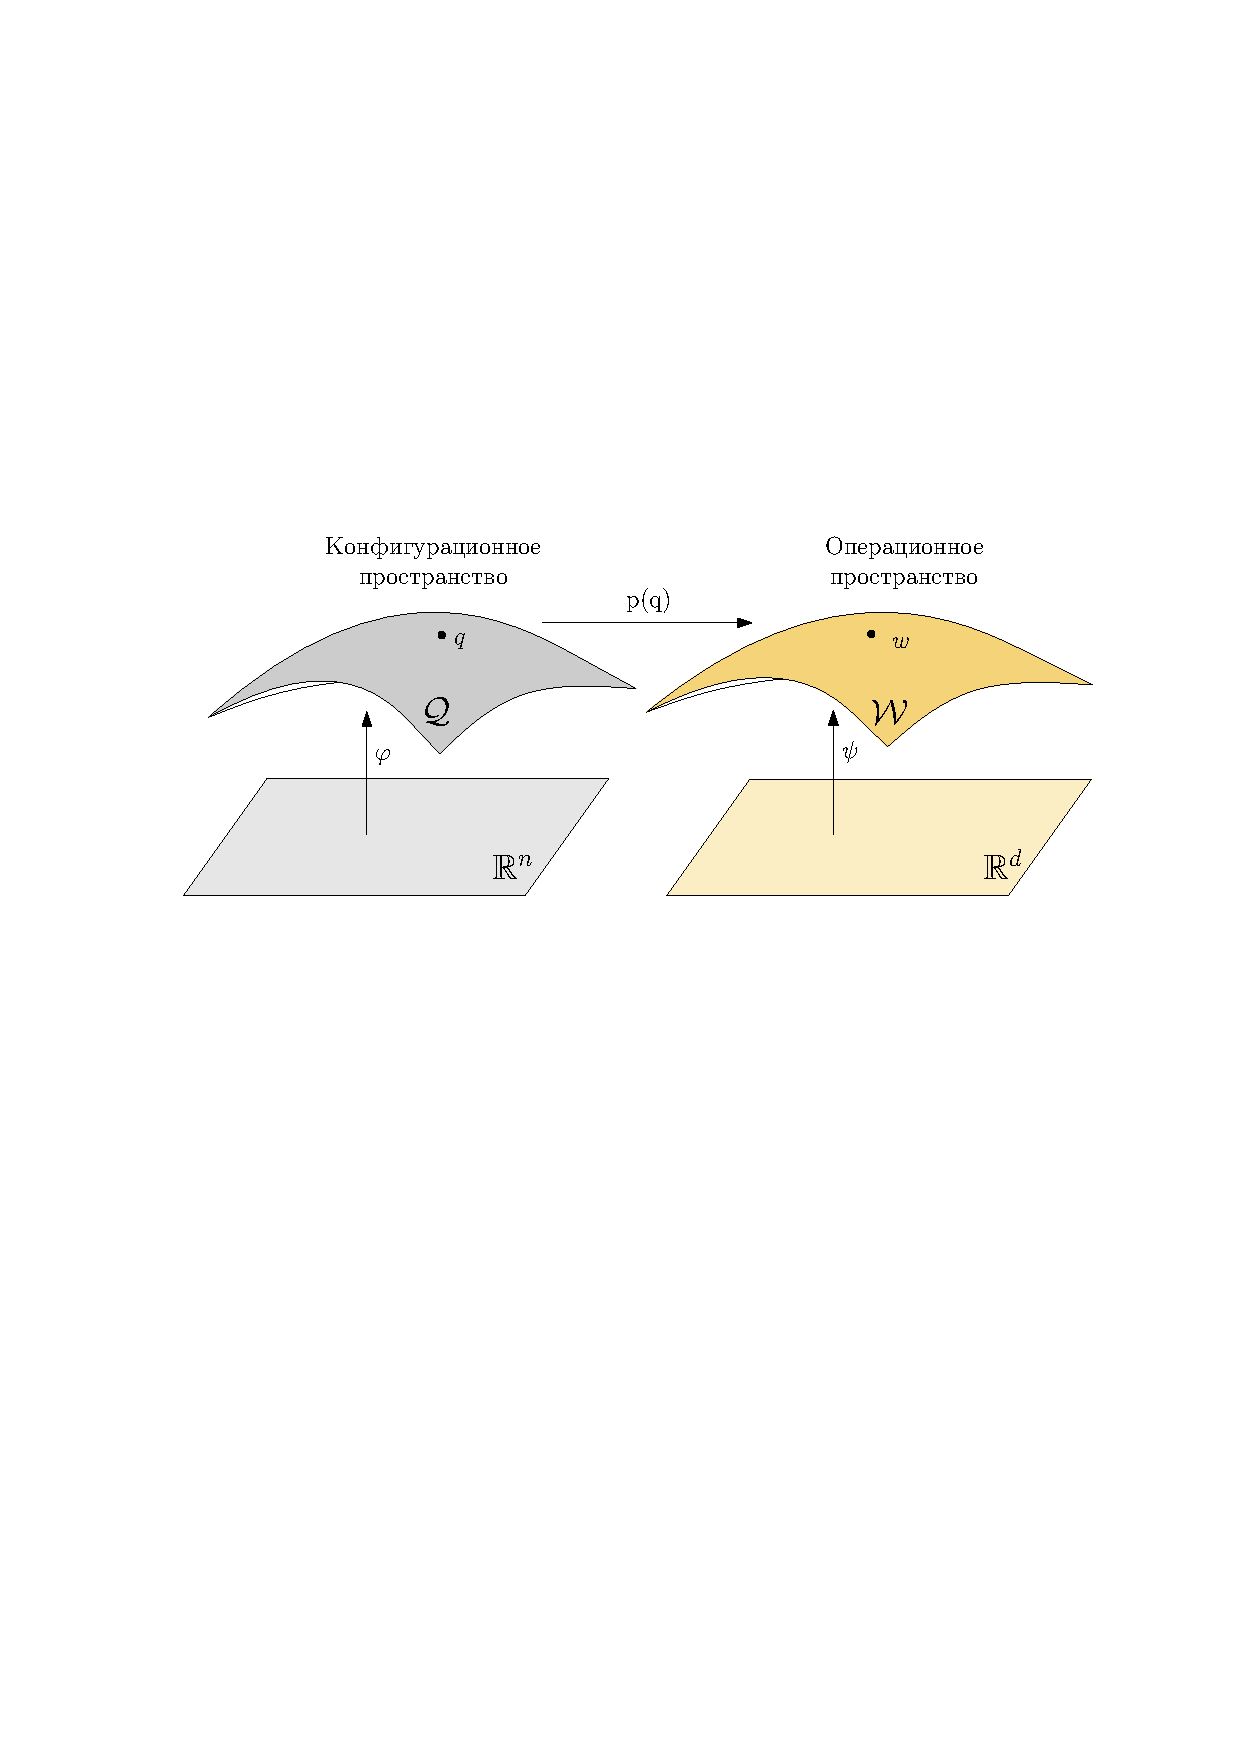
\includegraphics[width=1.0\textwidth]{figures/graph/manifolds.pdf}
                \label{fig:manifolds}
            \end{figure}
        \end{column}
        \begin{column}{0.42\textwidth}
            \begin{itemize}
                \item $w_i(q) = p_i(q) \in \mathcal{W} \subset \SE{3}$  --- трансформация из энд-эффектора $i$-го робота в базовую СК,
                \item $\psi: \SE{3} \rightarrow \R^6$
            \end{itemize}
        \end{column}
    \end{columns}
\end{frame}

\begin{frame}{Два манипулятора}
    \begin{equation}
        F(q) = \psi^{-1}(w^{-1}_1(q)w_2(q)), \quad q = \begin{bmatrix} q_1 & q_2\end{bmatrix}
    \end{equation}
    \begin{columns}
        \begin{column}{0.55\textwidth}
            \begin{figure}
                \centering
                % \animategraphics[loop,autoplay,width=1.0\linewidth]{3}{figures/gifs/plan_result-}{0}{31}
                \caption{Результат CBiRRT}
            \end{figure}
        \end{column}
        \begin{column}{0.42\textwidth}
            \begin{itemize}
                \item $w_i(q) = p_i(q) \in \mathcal{W} \subset \SE{3}$  --- трансформация из энд-эффектора $i$-го робота в базовую СК,
                \item $\psi^{-1}: \SE{3} \rightarrow \R^6$
            \end{itemize}
        \end{column}
    \end{columns}
\end{frame}


% \section{Результаты}
\begin{frame}{Результаты моделирования}
    \begin{itemize}
        \item Колличество эпизодов: 100
        \item Макс. время планирования: 60 с.
        \item $\varepsilon = 0.01$
    \end{itemize}
    \begin{table}[]
        \centering
        \begin{tabular}{|p{3cm}|c|c|c|c|c|}
        \hline
            \textbf{Критерий}& \textbf{CBiRRT} & \textbf{CPRM} &\textbf{CSST} &\textbf{CEST} & \textbf{BKPIECE1}\\
            \hline
            \textbf{Среднее стандартное отклонение от ограничения, м} & 0.0037 & 0.0028 & - & 0.0031 & 0.0028\\
            \hline
            \textbf{Среднее время планирования, сек} & 13.528 & 5.251915 & 60.0 & 13.84 & 21.75\\
            \hline
            \textbf{Успешность, \%} & 98 & 99 & 0 & 100 & 92\\
            \hline
        \end{tabular}
        \label{tab:my_label}
    \end{table}
\end{frame}

% \begin{frame}{Результаты}
%     \begin{figure}[ht]
%         \begin{subfigure}[b]{0.32\textwidth}
%             \centering
%             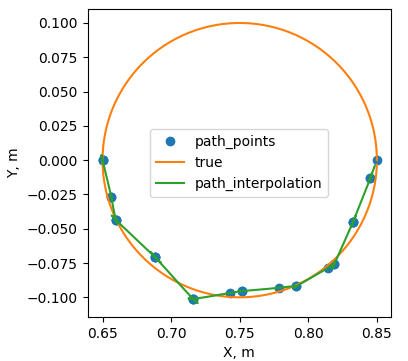
\includegraphics[width=0.9\textwidth]{figures/prm-result3.png}
%             \caption{CPRM}
%             \label{fig:rozum}
%         \end{subfigure}
%         \begin{subfigure}[b]{0.32\textwidth}
%             \centering
%             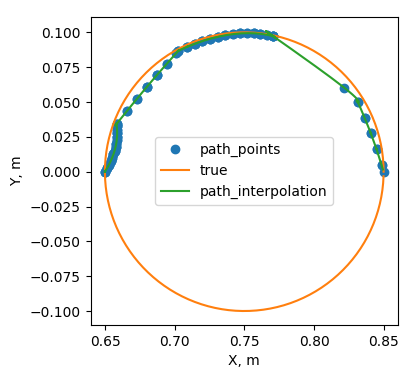
\includegraphics[width=0.9\textwidth]{figures/est-result1.png}
%             \caption{CEST}
%             \label{fig:ur}
%         \end{subfigure}
%         \begin{subfigure}[b]{0.32\textwidth}
%             \centering
%             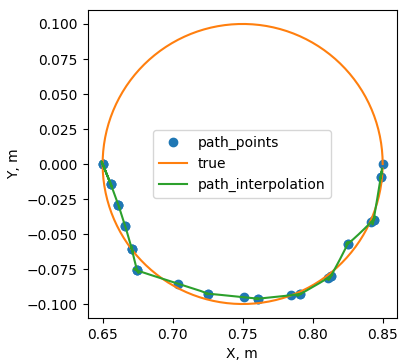
\includegraphics[width=0.9\textwidth]{figures/rrt-result1.png}
%             \caption{CBiRRT}
%             \label{fig:ur}
%         \end{subfigure}
%         \catpion{Результаты планирования}
%     \end{figure}
% \end{frame}

\begin{frame}{Заключение}
    \textbf{Выводы:}
    \begin{itemize}
        \item Проведен аналитический обзор методов
        \item Разработана среда моделирования для тестирования алгоритмов
        \item Реализованы алгоритмы \textit{CBiRRT}, \textit{TBRRT}, \textit{AtlasRRT}, \textit{RGDRRT}
    \end{itemize}
\end{frame}

\end{document}
